% vim: set tw=0:
\documentclass{beamer}
\usepackage{graphicx}
\usepackage{hyperref}
\hypersetup{pdfborder={0 0 0 0}}

% Reasonable themes:
% Antibes Bergen Berkeley Berlin Frankfurt Goettingen Ilmenau Luebeck Malmoe
% Montpellier PaloAlto Rochester Singapore Szeged Warsaw bars boxes
% compatibility default lined plain shadow sidebar split tree
% And these ones include the author's name on every slide:
% Berkeley

% Declare themes.
\mode<presentation>
\usetheme{UWHEP}

% Personal macros.
\newcommand{\email}[1]{{\texttt #1}}
\newcommand{\newframe}[1]{\section{#1}
    \frametitle{\sc{#1}}}
\newcommand{\subframe}[1]{\subsection{#1}
    \frametitle{\sc{#1}}}
\newcommand{\supers}[1]{\ensuremath{^\textrm{#1}}}
\newcommand{\subs}[1]{\ensuremath{_\textrm{#1}}}
\newcommand{\ca}{\ensuremath{\sim}}
\renewcommand{\email}[1]{\href{mailto:#1}{\nolinkurl{#1}}}

% Author information.
\title{T2 Status}
\author[Maier, Mohapatra]{
    Will Maier \and Ajit Mohapatra\\
    {\tt wcmaier@hep.wisc.edu}\\
    {\tt ajit@hep.wisc.edu}}
\institute[Wisconsin]{University of Wisconsin - High Energy Physics}
\date{2010.08.17}
\logo{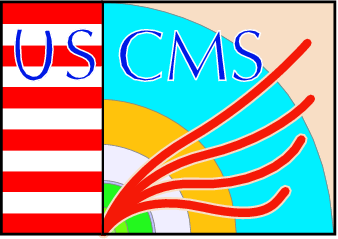
\includegraphics[height=0.6cm]{../../../Graphics/USCMS_logo.png}\hspace{.1cm}
\includegraphics[height=0.75cm]{../../../Graphics/UW_logo.png}}

\begin{document}

\begin{frame}
    \titlepage
\end{frame}

%\section{Overview}
%\begin{frame}
%    \tableofcontents
%\end{frame}

\section{Facilities}
\subsection{Software and Storage}
\begin{frame}
\frametitle{}

\begin{itemize}
  \item Deployed last of the 2x8 core Opteron 6136 servers
  \item Pool cleanup
  \item Downgraded 2x12 core Opteron 6176 SE test server to 6174
  \begin{itemize}
    \item CPUs hotter than AMD/Supermicro specified, failed vendor tests
    \item Too early for production deployment, will purchase 2x8 core Opteron 6136 again
  \end{itemize}
  \item Debugging PNFS timeouts
  \begin{itemize}
    \item Running on a ramfs (temporarily) cut down on timeouts drastically (but not completely)
    \item Tweaking PostgreSQL paramters changes timeout frequency, but they still happen
    \item Workload-dependent: when more than \ca{}10 jobs start per minute, some lookups start failing
  \end{itemize}
  \item Upgrading OSG worker node client to fix gLexec breakage
\end{itemize}
\end{frame}

\subsection{Production and Monitoring}
\begin{frame}
\frametitle{}

\begin{itemize}
    \item JobRobot: OK
    \item SAM: OK
    \item RSV: OK
    \item PhEDEx:
    \begin{itemize}
      \item Both Debug and Prod instances doing fine with 3\_3\_1
      \item Upgrade to 3\_3\_2 is planned this week
      \item No major transfer issues and lots of data transfer for local users.
      % 800 MB plot
    \end{itemize}
    \item MC Production:
    \begin{itemize}
      \item Summer10 finishing, Fall10 started
      \item Received 2 batches so far, total 320M
      \item Batch 1 is finishing (160M) and batch2 started; going ok so far, no major issues
      \item As usual US T2s and Omaha are doing fine, FNAL is now being used for production, too
    \end{itemize}
\end{itemize}
\end{frame}

\begin{frame}
  \begin{figure}
  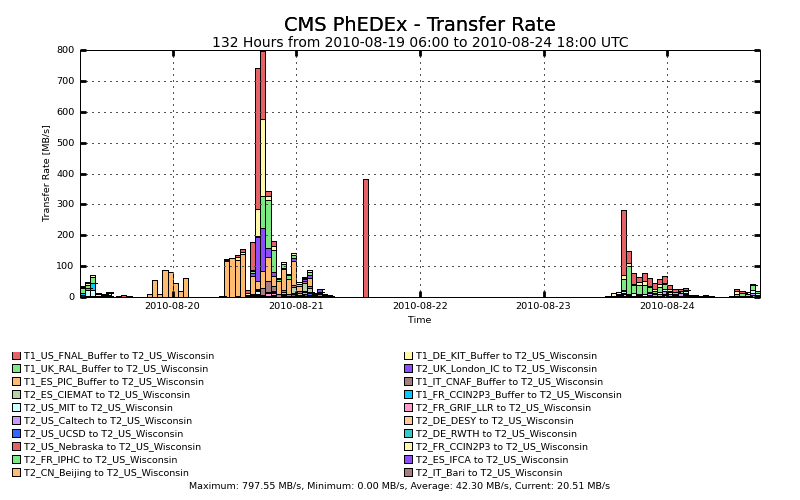
\includegraphics[height=6.5cm]{Graphics/phedex-rate-Aug2010.png}
  \caption{T2\_US\_Wisconsin PhEDEx transfer rates, August 2010}
  \end{figure}
\end{frame}


\end{document}
